% Generated by thesis/ch7/exp1/make_figures.py -- do not edit by hand.
\begin{figure}[p]
  \centering
  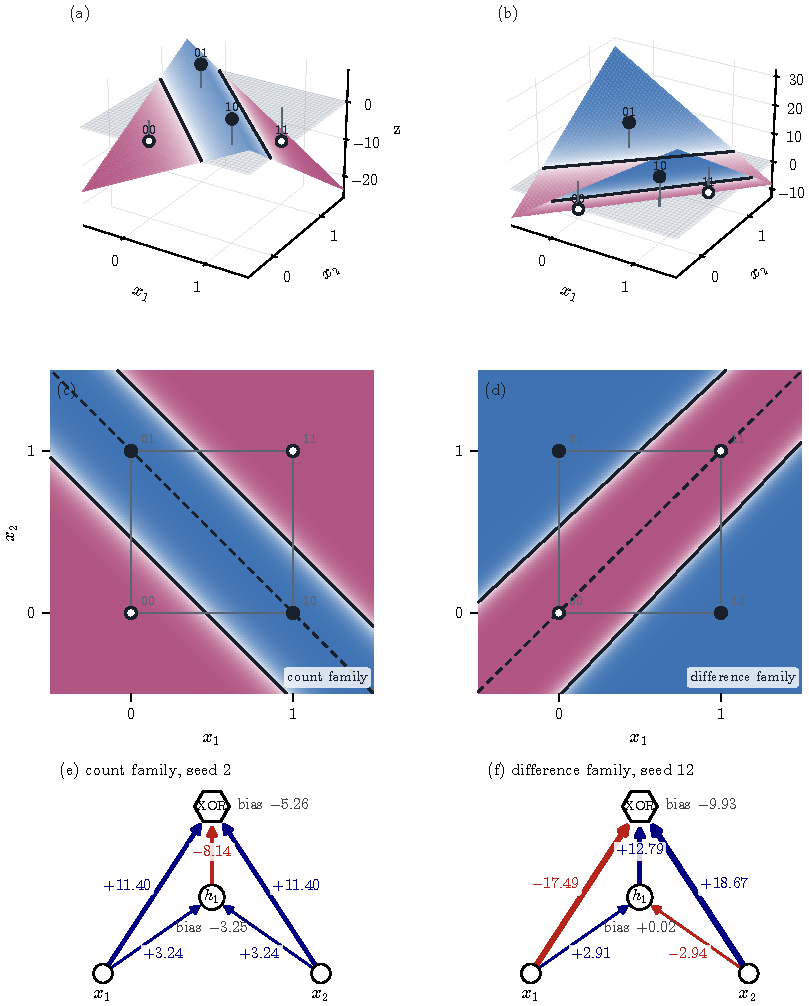
\includegraphics[width=\textwidth,height=0.77\textheight,keepaspectratio]{figures/ch7/xor-ridge-valley.pdf}
  \caption{XOR: one network of each family, the count family (a, c, e; seed 2) and the difference family (b, d, f; seed 12). (a, b) The score surface $z(x_1, x_2)$ over the plane $z = 0$ (grey); (c, d) the same scores from above. Shading: blue where the score is positive, magenta where it is negative, pale near 0; solid line: where it is 0. Filled points: the two inputs with XOR output 1; dashed line: the hidden unit's fold. (e, f) The networks of (a--d): circles $x_1$, $x_2$: the inputs; circle $h_1$: the hidden unit (ReLU); hexagon: the output unit, the logistic function of the score $z$. Edges: blue, a positive weight; red, a negative weight; thicker, a larger weight. The number on an edge is its weight; beside a unit, its bias.}
  \label{fig:ch7-xor-ridge-valley}
\end{figure}
